\documentclass[a4paper, 11pt]{book}
\usepackage{/home/nicolas/Documents/Enseignement/Prepa/bpep/fichiers_utiles/preambule}

\newcommand{\dsNB}{8}
\makeatletter
\renewcommand{\@chapapp}{Kh\^olles MPSI3 -- semaine \dsNB}
\makeatother

\toggletrue{corrige}  % décommenter pour passer en mode corrigé

\begin{document}

\resetQ
\newpage

\chapter{Sujet 1\siCorrige{\!\!-- corrig\'e}}

\section{Question de cours}

Définir la quantité de matière, la masse molaire et son lien avec la quantité de
matière, les fractions molaire et massique, les concentrations molaire et
massique et le lien entre les deux.

\subimport{/home/nicolas/Documents/Enseignement/Prepa/bpep/exercices/Colle/circuit_RLC_serie/}{sujet.tex}

\resetQ
\newpage

\chapter{Sujet 2\siCorrige{\!\!-- corrigé}}
\section{Question de cours}

Refaire l'exercice sur les fractions molaire et massique de dioxygène et
diazote, l'exemple sur la concentration molaire de $\ce{Na+}$~:
\begin{tcbraster}[raster columns=2, raster equal height=rows]
    \begin{NCexem}[width=\linewidth]{Exercice}
        L'air est constitué, en quantité de matière, à 80\% de diazote N$_2$ et
        à 20\% de dioxygène O$_2$. On a $M({\rm N_2}) = \SI{28.0}{g.mol^{-1}}$
        et $M({\rm O_2}) = \SI{32.0}{g.mol^{-1}}$. En déduire les fractions
        molaires puis les fractions massiques.
    \end{NCexem}
    \begin{NCexem}[]{Exercice}
        On dissout une masse $m = \SI{2.00}{g}$ de sel NaCl$\sol$ dans $V =
        \SI{100}{mL}$ d'eau. \textbf{Déterminer la concentration en
        Na$\plus{}$ dans la solution}. ($M(\ce{NaCl}) = \SI{58.44}{g.mol^{-1}}$)
    \end{NCexem}
\end{tcbraster}

\subimport{/home/nicolas/Documents/Enseignement/Prepa/bpep/exercices/Colle/regime_transitoire_ordre2/}{sujet.tex}

\resetQ
\newpage

\chapter{Sujet 3\siCorrige{\!\!-- corrigé}}
\section{Question de cours}

Réaction totale et avancement maximal~: refaire l'exemple du cours sur la
combustion du méthane $\ce{CH4\gaz{} + 2O2\gaz{} \rightarrow CO2\gaz{} +
2H2O\gaz{}}$ avec $n_{\ce{CH4}}^0 = \SI{2}{mol}$ et $n_{\ce{O2}}^0 =
\SI{3}{mol}$.

\resetQ
\section{Circuit de \textsc{Wien}}

\begin{minipage}{0.60\linewidth}

    On réalise le montage suivant. On ferme l'interrupteur à l'instant $t =0$,
    $C$ traversé par $i'$ étant initialement chargé et $C$ traversé par $i$
    étant initialement déchargé.\smallbreak
    On pose $\tau = RC$. Données~: $R = \SI{10}{k\ohm}$ et $C = \SI{0.1}{\micro
    F}$.
\end{minipage}
\begin{minipage}{0.40\linewidth}
    \centering
    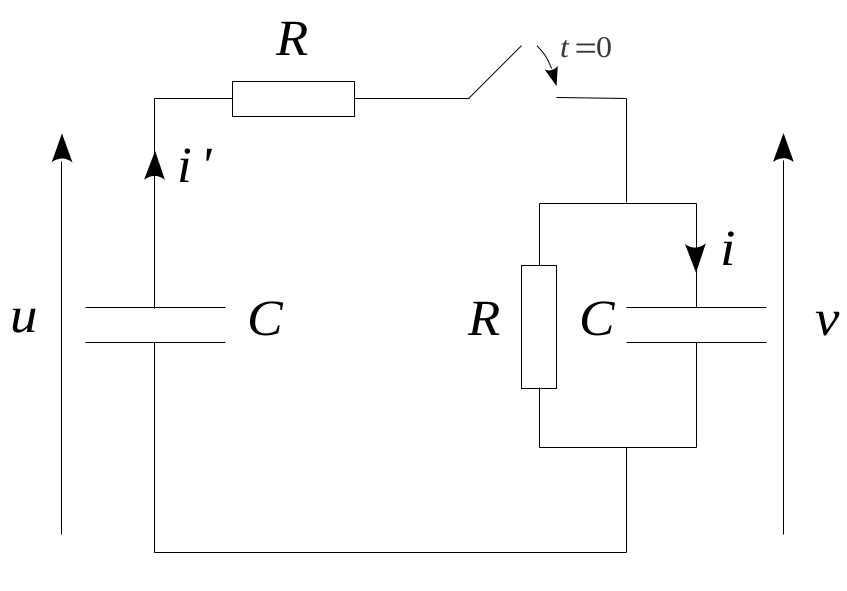
\includegraphics[width=\linewidth]{wien}
\end{minipage}

\QR{À partir de considérations physiques, préciser les valeurs de la tension $v$
    lorsque $t = 0$ et $t = \infty$.
}{
    Le condensateur de tension $v$ est indiqué être initialement déchargé, on a
    donc $v(0^-) = 0$. Comme un condensateur est de tension continue, on a donc
    \fbox{$v(0^+) = 0$}. De plus, à $t \longrightarrow \infty$, les deux
    condensateurs seront forcément déchargés à cause des résistances dissipant
    l'énergie, il ne peut y avoir conservation~: il seront donc équivalent à des
    interrupteurs ouverts, et on aura donc notamment \fbox{$v(\infty) = 0$}.
}

\QR{
    Établir l'équation différentielle du second ordre dont la tension $v$ est
    solution.
}{
    Avec une loi des mailles, on a
    \[ u = v+Ri'\]
    Or, la RCT du condensateur de gauche \textbf{en convention générateur} est
    \[i' = -C \diff{u}{t} \Rightarrow i' = -C \diff{v}{t} - RC \diff{i'}{t}\]
    On a donc une équation avec $\diff{v}{t}$. On cherche donc à exprimer $i'$ en
    fonction de $v$, ce que l'on fait avec la loi des nœuds et les RCT du
    condensateur de droite $i = C \diff{v}{t}$ et de la résistance $R(i'-i) = v$~:
    \begin{equation}\label{eq:wieni}
        i' = i + \frac{v}{R} \Leftrightarrow i' = C \diff{v}{t} + \frac{v}{R}
    \end{equation}
    En combinant les deux, on a
    \begin{gather*}
        C \diff{v}{t} + \frac{v}{R} =
            -C \diff{v}{t} - RC \diff{}{t} \left( C \diff{v}{t} + \frac{v}{R} \right)
        \Leftrightarrow
        C \diff{v}{t} + \frac{v}{R} =
            -C \diff{v}{t} - RC^2 \diff[2]{v}{t} - C \diff{v}{t}\\
        \Leftrightarrow
        \diff[2]{v}{t} + \frac{3}{RC} \diff{v}{t} + \frac{v}{(RC)^2} = 0
        \Leftrightarrow
        \boxed{\diff[2]{v}{t} + \frac{3}{\tau} \diff{v}{t} + \frac{v}{\tau^2} = 0}
    \end{gather*}
}

\QR{
    En déduire l'expression de $v(t)$ en déterminant les
    constantes d'intégration.
    
}{
    On écrit l'équation caractéristique de discriminant $\Delta$~:
    \begin{gather*}
        r^2 + \frac{3}{\tau}r + \frac{1}{\tau^2} = 0 \Rightarrow \Delta =
        \frac{9}{\tau^2} - \frac{4}{\tau^2} = \frac{5}{\tau^2} > 0\\
        \Longrightarrow r_\pm = - \frac{3}{2\tau} \pm \frac{\sqrt{5}}{2\tau} < 0
    \end{gather*}
    On a donc un régime apériodique, dont les solutions générales sont
    \[\boxed{v(t) = A\text{e}^{r_+t} + B\text{e}^{r_-t}}\]
    En finissant la détermination des constantes d'intégration, on trouve
    \begin{equation*}
        \boxed{v(t) = \frac{E}{\tau(r_+ - r_-)}
                      \left[ \text{e}^{r_+t} - \text{e}^{r_-t} \right]}
    \end{equation*}
}

\QR{Donner l'allure du graphe correspondant à $v(t)$. 
}{
    \begin{minipage}{0.49\linewidth}

        Le condensateur est initialement chargé. Soit $E$ sa tension initiale.
        On utilise l'équation~\ref{eq:wieni} pour trouver que $\diff{v}{t} (0) =
        \frac{i' (0)}{C}$, sachant qu'à $t = 0$ le circuit est équivalent à un
        circuit $RC$ en décharge et qu'on a donc $i'(0) = E/R$. On trouve ainsi
        \[\boxed{\diff{v}{t} (0) = \frac{E}{\tau}}\]
        \hfill
    \end{minipage}
    \begin{minipage}{0.49\linewidth}
        \begin{center}
            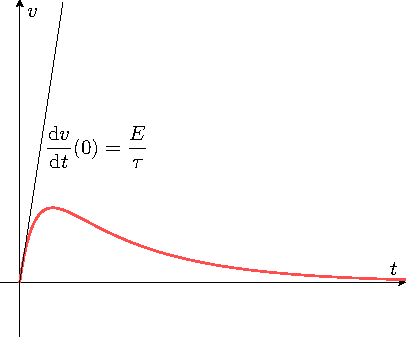
\includegraphics[width=\linewidth]{wien_carac}
        \end{center}
    \end{minipage}
}

\end{document}
